\section{Timing and Calibration}
\subsection{Clock convention and measurement density}
We align the logs on the Pi monotonic clock. Its calendar was incorrect during recording, so original folder dates serve only as identifiers. We take the camera exposure window as $[t_s-T,t_s]$, interpreting $t_s$ as the first-row readout/exposure-end timestamp and $T$ as the recorded exposure. Rolling-row timing was not measured. Depth and screen logs use host receipt times; the saved device ticks and player clock were not calibrated to this timebase.

Each selected coded exposure contains 10--11 valid received depth frames in one second. We take the median of the central four zones (rows 4--5, columns 4--5, one-based), requiring at least three positive zones, depth 200--2000\,mm and within-region spread no greater than 50\,mm. We omit the known startup sample and interpolate between received frames. Raw depth is used without subtracting the 22\,mm base-to-paper offset.

\begin{figure*}[t]
\centering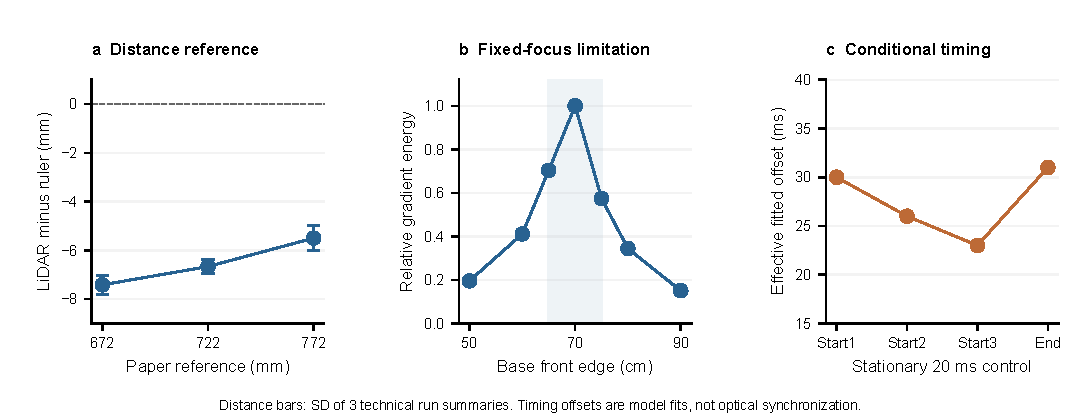
\includegraphics[width=\textwidth]{images/acquisition_bounds.pdf}
\caption{Acquisition checks. (a) Depth residual against the paper reference, including the 22\,mm base-to-paper offset. Bars show sample SDs of three technical run summaries; optical-origin uncertainty remains. (b) Registered gradient energy relative to 70\,cm shows fixed-focus variation. It is a proxy of sharpness but it does not measure the resolution. The range 65--75\,cm base that was kept for use is shaded. (c) Short-exposure controls give fitted offset (effective); the optical synchronization was not measured.}
\label{fig:bounds}
\end{figure*}

\subsection{Stationary checks}
At paper references 672, 722 and 772\,mm, three technical run summaries give depths of $664.58\pm0.38$, $715.33\pm0.29$ and $766.50\pm0.50$\,mm (mean $\pm$ sample SD). The residuals are $-7.42$, $-6.67$ and $-5.50$\,mm. One near-labelled record matches the far position. It is retained as a position/reference discrepancy but excluded from this summary. Given that the origin in the optical data is not defined, the residual cannot be attributed completely to sensor errors.

\Needspace{14\baselineskip}
Stationary 19.969\,ms controls give fitted screen offsets of 30, 26 and 23\,ms initially, and 31\,ms at the end (end-fit $R^2=0.985$). We use 26\,ms as an effective command-to-image offset. Each one-second control has only six covered observations, with weaker transferred-fit agreement ($R^2=0.814$, 0.607, 0.525). The short-exposure fit therefore leaves uncertainty in the long-exposure illumination history. The fixed-patch black/white raw-intensity ratio varies from about 0.167 to 0.211; we use 0.19 in the main model.

Relative gradient energy is 0.70 at 65\,cm and 0.57 at 75\,cm, compared with 70\,cm. It falls to 0.20 and 0.15 at 50 and 90\,cm (Fig.~\ref{fig:bounds}). These fixed-focus checks led us to restrict motion to the narrower range, where some defocus still remains. The selected motion images and final controls are unclipped; two initial white controls each contain one clipped raw pixel. The reference is the median of ten static 100\,ms frames at the nominal 70\,cm base position. These frames form one reference, not ten independent experimental repeats.
